\documentclass[11pt,border=5pt]{standalone}
\usepackage{fontspec}
\setmainfont{cmunrm.otf}[BoldFont=cmunbx.otf,ItalicFont=cmunti.otf,BoldItalicFont=cmunbi.otf]
\usepackage{amsmath}
\usepackage{unicode-math}
\setmathfont{NewCMMath-Regular.otf}
\usepackage{tikz}
\usetikzlibrary{arrows.meta,patterns,angles,quotes}
\begin{document}
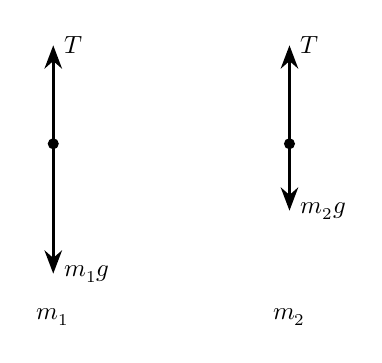
\begin{tikzpicture}[>=Stealth,font=\small,line cap=round,line join=round]
\fill (0,0) circle (2pt);
\draw[->,very thick] (0,0) -- (0,1.25) node[right] {$T$};
\draw[->,very thick] (0,0) -- (0,-1.65) node[right] {$m_1g$};
\begin{scope}[xshift=3cm]\fill (0,0) circle (2pt);
\draw[->,very thick] (0,0) -- (0,1.25) node[right] {$T$};
\draw[->,very thick] (0,0) -- (0,-0.85) node[right] {$m_2g$};
\end{scope}\node at (0,-2.2) {$m_1$};
\node at (3,-2.2) {$m_2$};

\end{tikzpicture}
\end{document}
